%  Copyright (C) 2003 David Roundy
%
%  This program is free software; you can redistribute it and/or modify
%  it under the terms of the GNU General Public License as published by
%  the Free Software Foundation; either version 2, or (at your option)
%  any later version.
%
%  This program is distributed in the hope that it will be useful,
%  but WITHOUT ANY WARRANTY; without even the implied warranty of
%  MERCHANTABILITY or FITNESS FOR A PARTICULAR PURPOSE.  See the
%  GNU General Public License for more details.
%
%  You should have received a copy of the GNU General Public License
%  along with this program; if not, write to the Free Software Foundation,
%  Inc., 59 Temple Place - Suite 330, Boston, MA 02111-1307, USA.  
\documentclass[floats]{report}
\usepackage{color}
\usepackage{epsfig}
\usepackage{amsmath, amsthm, amssymb}

\usepackage{html}

\begin{document}

% Definition of title page:
\title{
    Dactyl\\
{\Large \it CYLindric Time DomAin}
}
\author{
    David Roundy, Mihai Ibanescu, Peter Bermel
}

\maketitle 

\tableofcontents

\chapter{The Yee lattice}

\begin{figure}
\caption{Yee lattice in cylindrical coordinates.
\label{yee_fig}}
\centering
\mbox{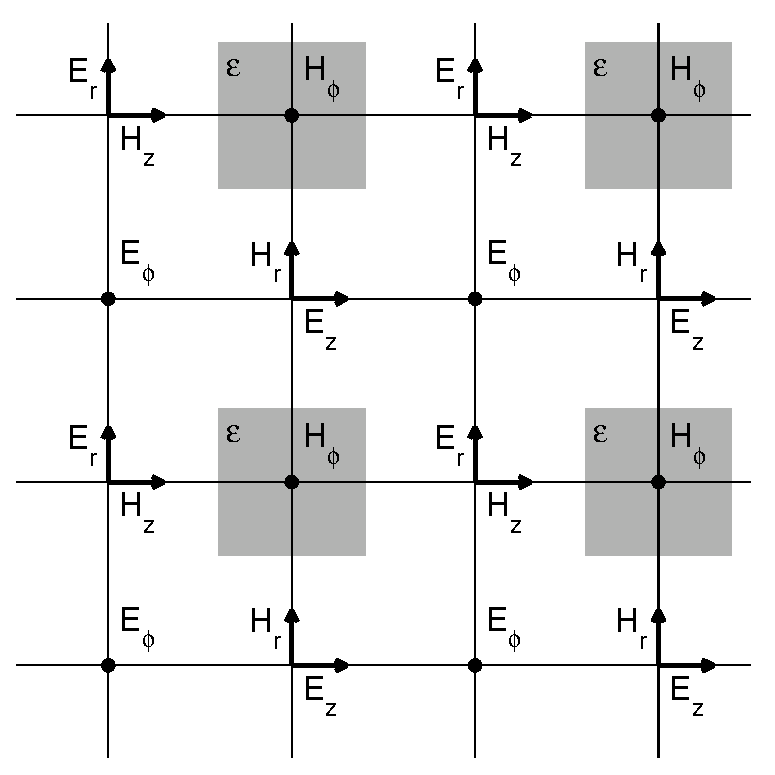
\epsfig{file=Yee_bulk.eps,width=7.8cm}}
\vspace{13cm}
\end{figure}

\chapter{Maxwell's equations in cylindrical coordinates}

Here are Maxwell's equations in cylindrical coordinates.  We take the
fields to be of the form:
\begin{equation*}
\mathbf{E}(r,\phi,z) = \mathbf{E}_m(r,z)e^{i m \phi} 
\end{equation*}

Without further ado:
\begin{align}
\frac1c\frac{dH_r}{dt} &= \frac{dE_\phi}{dz} - \frac{im}r E_z\\
\frac1c\frac{dH_\phi}{dt} &= \frac{dE_z}{dr} - \frac{dE_r}{dz}\\
\frac1c\frac{dH_z}{dt} &= \frac{im}r E_r - \frac1r\frac{d(rE_\phi)}{dr}
\end{align}
\begin{align}
\frac\epsilon c\frac{dE_r}{dt} &= \frac{im}r H_z - \frac{dH_\phi}{dz} \\
\frac\epsilon c\frac{dE_\phi}{dt} &= \frac{dH_r}{dz} - \frac{dH_z}{dr} \\
\frac\epsilon c\frac{dE_z}{dt} &= \frac1r\frac{d(rH_\phi)}{dr} - \frac{im}r H_r
\end{align}


\chapter{PML}

PML (Perfectly Matched Layers) is used to provide absorbing boundary
conditions in either the $z$ or $r$ direction.  PML consists of a material
in which some of the field components are split into two fields, each of
which has a conductivity associated with it, which is responsible for the
absorption of the PML.

PML is a sort of material that contains a set of conductivities $\sigma_r$,
$\sigma_\phi$ and $\sigma_z$.  These conductivities are both $\mathbf{E}$
and $\mathbf{H}$ conductivities---yes, we have magnetic monopoles moving
around in our PML.  $\ddot\smile$ Each $\sigma$ causes absorption of
radiation in the direction it is named after.  Thus $\sigma_\phi$ is small,
and almost unnecesary, and is only needed because of the curvature of the
radial surface.  The value of $\sigma_\phi$ at a given radius is equal to
\begin{equation}
\sigma_\phi(r) = \frac1r \int_0^r \sigma_r(r)dr
\end{equation}

If we had a IDTD (Infinitesimal Difference Time Domain) code, PML would be
perfectly absorbing, regardless of the variation of $\sigma$ with position.
However, since dactyl is a lowly FDTD code, we have to make sure that
$\sigma$ varies only slowly from one grid point to the next.  We do this by
making $\sigma_z$ (for example) vary as $z^2$, with a maximum value of
$\sigma_{max}$ right in front of the boundary.  At the edge of the PML
region is a metalic boundary condition.  The optimal value of
$\sigma_{max}$ is determined by a tradeoff between reflection off the
metallic boundary, caused by too little a $\sigma_{max}$, and reflection
off the sigma itself, caused by too large a $\sigma_{max}$, which makes for
a large variation of $\sigma$ from one grid point to the next.

Here are the field equations for a PML material:
\begin{align}
\frac{dH_{r\phi}}{dt} &= - c \frac{im}r E_z             - \sigma_\phi H_{r\phi} &
\frac{dH_{rz}}{dt} &= c \frac{dE_\phi}{dz}              - \sigma_z H_{rz}\\
\frac{dH_{\phi z}}{dt} &= - c \frac{dE_r}{dz}           - \sigma_z H_{\phi z} &
\frac{dH_{\phi r}}{dt} &= c \frac{dE_z}{dr}             - \sigma_r H_{\phi r} \\
\frac{dH_{zr}}{dt} &= - c \frac1r\frac{d(rE_\phi)}{dr}  - \sigma_r H_{zr}  &
\frac{dH_{z\phi}}{dt} &= c \frac{im}r E_r               - \sigma_\phi H_{z\phi} \\
\epsilon\frac{dE_{r\phi}}{dt} &=   c \frac{im}r H_z             - \sigma_\phi E_{r\phi} &
\epsilon\frac{dE_{rz}}{dt} &= -c\frac{dH_\phi}{dz}              - \sigma_z E_{rz}\\
\epsilon\frac{dE_{\phi z}}{dt} &=   c \frac{dH_r}{dz}           - \sigma_z E_{\phi z} &
\epsilon\frac{dE_{\phi r}}{dt} &=-c \frac{dH_z}{dr}             - \sigma_r E_{\phi r} \\
\epsilon\frac{dE_{zr}}{dt} &=   c \frac1r\frac{d(rH_\phi)}{dr}  - \sigma_r E_{zr}  &
\epsilon\frac{dE_{z\phi}}{dt} &=-c \frac{im}r H_r               - \sigma_\phi E_{z\phi} 
\end{align}

\appendix

\input{gpl.tex}

\end{document}

